%
% File acl2012.tex
%
% Contact: Maggie Li (cswjli@comp.polyu.edu.hk), Michael White (mwhite@ling.osu.edu)
%%
%% Based on the style files for ACL2008 by Joakim Nivre and Noah Smith
%% and that of ACL2010 by Jing-Shin Chang and Philipp Koehn


\documentclass[11pt,letterpaper]{article}
\usepackage[letterpaper]{geometry}
\usepackage{acl2012}
\usepackage{times}
\usepackage{latexsym}
\usepackage{graphicx}
\usepackage{amssymb}
\usepackage{amsmath}
\usepackage{multirow}
\usepackage{url}
\makeatletter
\newcommand{\@BIBLABEL}{\@emptybiblabel}
\newcommand{\@emptybiblabel}[1]{}
\makeatother
\usepackage[hidelinks]{hyperref}
\DeclareMathOperator*{\argmax}{arg\,max}
\setlength\titlebox{6.5cm}    % Expanding the titlebox

\title{Discovering Cognates Using LSTM Networks}

% \author{First Author \\
%   Affiliation / Address line 1 \\
%   Affiliation / Address line 2 \\
%   Affiliation / Address line 3 \\
%   {\tt email@domain} \\\And
%   Second Author \\
%   Affiliation / Address line 1 \\
%   Affiliation / Address line 2 \\
%   Affiliation / Address line 3 \\
%   {\tt email@domain} \\}

\author{Shantanu Kumar \and Ashwini Vaidya \and Sumeet Agarwal \\ 
  Indian Institute of Technology Delhi
  \\ {\tt \{ee1130798, ird11278, sumeet\}@iitd.ac.in}}

\date{}

\begin{document}
\maketitle

%%%%%%%%%%%%%%%%%%%%%%%%%%%%%%%%%%%%%%%%%%%%%%%%
\begin{abstract}
In this paper, we present a deep learning (DL) model for the task of pairwise cognate prediction. We use a character level model with recurrent neural network architecture and attention. We compare the performance of our model with previous approaches on various language families. We are able to show that our model performs better than non-DL methods which exploit surface similarity measures as well as a recent convolutional neural network (CNN) based model for the task. We also employ our model specifically to the domain of discovering cognates from Hindi-Marathi to assist the task of lexical resource creation.
\end{abstract}

%%%%%%%%%%%%%%%%%%%%%%%%%%%%%%%%%%%%%%%%%%%%%%%%
\section{Introduction}
Cognates are words across different languages that are known to have originated from the same word in a common ancestral language. For example, the English word `\textit{Night}' and the German word `\textit{Nacht}', both meaning \textit{Night} and English `\textit{Hound}' and German `\textit{Hund}', meaning \textit{Dog} are cognates whose origin can be traced back to Proto-Germanic. Cognate words are not simply the translations of each other in any two languages, but are historically known to have a common origin. For example, the English word `\textit{Hound}' and the Spanish word `\textit{Perro}' both mean \textit{Dog} but are not cognates.

Traditionally, the identification of cognates was carried out by historical linguists, using word lists and establishing sound correspondences between words. These are useful in determining linguistic distance within a language family, and also to understand the process of language change. Cognate information has also been used in several downstream NLP tasks, like sentence alignment in bi-texts \cite{simard1993using} and improving statistical machine translation models \cite{kondrak2003cognates}. Additionally, it has been proposed that cognates can be used to share lexical resources among languages that are closely related \cite{Singh:07b}.

For some time now, there has been a growing interest in automatic cognate identification techniques. Most approaches for this task focus on finding similarity measures between a pair of words such as orthographic or phonetic similarity \cite{hauer2011clustering} \cite{inkpen2005similarity} \cite{List2016g}. These are used as features for a classifier to identify cognacy between a given word-pair. Surface similarity measures miss out on capturing generalizations beyond string similarity, as cognate words are not always revealingly similar. \cite{rama2015automatic} attempt to identify cognates by looking at the common subsequences present in the candidate word pair. For a cognate pair like the English `\textit{Wheel}' and the Sanskrit `\textit{Chakra}', such an approach fails as they have nothing in common with each other orthographically. In fact, even for a pair like English `\textit{Father}' and Latin `\textit{Pater}', a common subsequence approach completely ignores the similarity between the `\textit{Fa}' and `\textit{Pa}' phonemes, which is a possible indication of cognacy between the pair. Thus, there is a need of information about phonological similarity that is beyond surface similarity, such as the sound correspondences that are used in historical linguistics to narrow down candidate pairs as cognates.

By using DL based models, the need for external feature engineering is circumvented as the system learns to find hidden representations of the input depending on the task in hand. Our paper presents an end-to-end character-level recurrent neural network (RNN) based model that is adapted from a model used on a similar word-level task called RTE \cite{rocktaschel2016reasoning}. Our model is able to outperform both the common subsequence model \cite{rama2015automatic} as well as a recent CNN-based model \cite{rama2016siamese} on the task. 

LSTM (Long Short Term Memory) networks are being used in an extensive range of NLP tasks to build end-to-end systems. LSTMs have been successfully applied to machine translation \cite{bahdanau2014neural}. language modeling \cite{mikolov2010recurrent}, information retrieval \cite{sordoni2015hierarchical} and RTE \cite{snli:emnlp2015}. In the subsequent sections, we describe our LSTM based Siamese-style architecture which uses character by character attention to enrich the representations of the input word pairs and make the cognate prediction. We perform thorough analysis on the performance of our model and compare it against existing supervised approaches, including the subsequence based model \cite{rama2015automatic}.

%A key observation is that language-based features either with respect to language family or phonetic relationships does not help performance, while semantic information has a positive effect. We find that pre-training on language data unrelated to the language family is also useful, which points to the model's flexibility and its ability to capture statistical regularities without explicit feature engineering.

% We also compare our model's performance with existing supervised approaches, including the subsequence model described in \cite{rama2015automatic} (and its variants). Even if these models are provided with richer character representations in the form of IPA encoding, they are still unable to identify cognate pairs from very broad cognate classes. On the other hand, the LSTM model, even when pre-trained with data from a completely unrelated language family has a much lower error rate.  \textit{Some lines need to be added here about the result pairs}

The task of discovering cognates can possibly be particularly useful among the languages of South Asia, which are not rich in lexical resources. Information about cognates can become an important source for assisting the creation and sharing of lexical resources between languages. Therefore, another contribution of this work is to apply our cognate detection model to a real language pair. We apply our model to the domain of Hindi-Marathi, using a large unlabeled corpus of aligned texts to find cognate pairs.

%%%%%%%%%%%%%%%%%%%%%%%%%%%%%%%%%%%%%%%%%%%%%%%%
% \section{Related Work}

% There have been several previous works for automatic cognate identification that try to exploit different forms of features and representations for capturing the necessary information.

% \textbf{Orthographic features based classifier} : \cite{hauer2011clustering} use a number of basic word similarity measures as input to a SVM classifier for cognate prediction. They use features like common bigrams, longest common substring, word length difference etc. The also use features that encode the degree of affinity between pairs of languages.

% \textbf{Gap-weighted common subsequences} : \cite{rama2015automatic} uses a string kernel based approach wherein he defines a vector for a word pair using all common subsequences between them and weighting the subsequence by their gaps in the strings. The subsequence based features outperform orthographic word similarity measures.

% \textbf{Siamese ConvNet model} : In a recent work, T. Rama introduces CNN based siamese-style model \cite{rama2016siamese} for the task. The model is inspired by image-similarity CNN models. Instead of CNNs, we propose the use of LSTM networks. As these are a form of recurrent network (RNN), they fit more naturally to natural language which also has a sequential architecture and follows a linear order. In comparison, convolutional networks are more hierarchical and hence seem natural for images. Even though NLP literature does not support a clear distinction between the domains where CNNs or RNNs perform better, recent works have shown that each provide complementary information for text classification tasks \cite{yin2017comparative}. 

%We do an extensive analysis of our trained models to try to understand the kinds of features it learns to recognize that are important for making the cognate judgements.

%By using deep learning based models, the need for external feature engineering is avoided and the system outperforms previous works for cognate detection.


%%%%%%%%%%%%%%%%%%%%%%%%%%%%%%%%%%%%%%%%%%%%%%%%
\section{Datasets}

The task of cognate identification will make use of word lists of different language families taken from the basic vocabulary e.g. kinship terms, body parts, numbers etc. Usually this vocabulary will represent concepts from the language itself and not borrowed items, (although this is also possible at times). A word list can be considered as a table where the different rows and columns represent different languages and concepts respectively. Each cell in the table contains a lexical item along with its cognate class ID which helps to determine if two words are cognates.

We make use of three datasets in our work which come from three different language families. These families make a good test set as they vary widely in terms of the number of languages, concepts and cognate classes. The first and primary dataset that we use is the IELex Database, which contains cognacy judgements from the Indo-European language family. The dataset is curated by Michael Dunn\footnote{http://ielex.mpi.nl/}. Second, we include a dataset taken from the Austronesian Basic Vocabulary project \cite{greenhillBlust:08}, and a third dataset from the Mayan family \cite{wichmann:2008}. 

There are several differences in transcription in each of these datasets. While IELex is available in both IPA and a coarse `Romanized' IPA encoding, the Mayan database is available in the ASJP format (similar to a Romanized IPA) \cite{Brown:08} and the Austronesian has been semi-automatically converted to ASJP \cite{rama2016siamese}. We use subsets of the original databases due to lack of availability of uniform transcription.

The IELex database contains words from 52 languages for over 200 concepts, while the Austronesian contains words from 100 languages and as many concepts. The Mayan dataset is comparatively very small with only 100 concepts from 30 languages. The Austronesian dataset also contains the largest number of cognate classes as compared to the other two. The number of samples obtained from each dataset are mentioned in Tables~\ref{CL_count} and \ref{CC_count}. The small size of the Mayan dataset especially poses a challenge for training the deep learning networks which is addressed in the later sections. 

We also use the TDIL Hindi-Marathi sentence-aligned corpus as the large unlabeled data for our final model. This dataset provides a large part of the vocabulary from the both the languages to search for cognates.


% %%%%%%%%%%%%%%%%%%%%%%%%%%%%%%%%%%%%%%%%%%%%%%%%
% \section{Gap-weighted subsequence model}
% Before coming to the LSTM based model, we performed a thorough analysis on the performance of the gap-weighted subsequence model.
% There were two fundamental drawbacks in using the common-subsequence model (Referred to as \textit{Multiplicative} model). 

% Firstly, since the model only looked at common subsequences, it ignored vital information about closely related subsequences such as \textit{`fa'} in FATHER and \textit{`pa'} in PATER which are cognate words. 
% Secondly, this also resulted in very sparse vectors as the feature space size was huge. To overcome these problems, we tried smoothing techniques which resulted in models Hy-Avg, Hy-Norm and Additive.

% \subsection{Error Analysis}

% \subsection{Modified model}

%%%%%%%%%%%%%%%%%%%%%%%%%%%%%%%%%%%%%%%%%%%%%%%%
\section{Approach}

\begin{figure}[t]
	\centering
	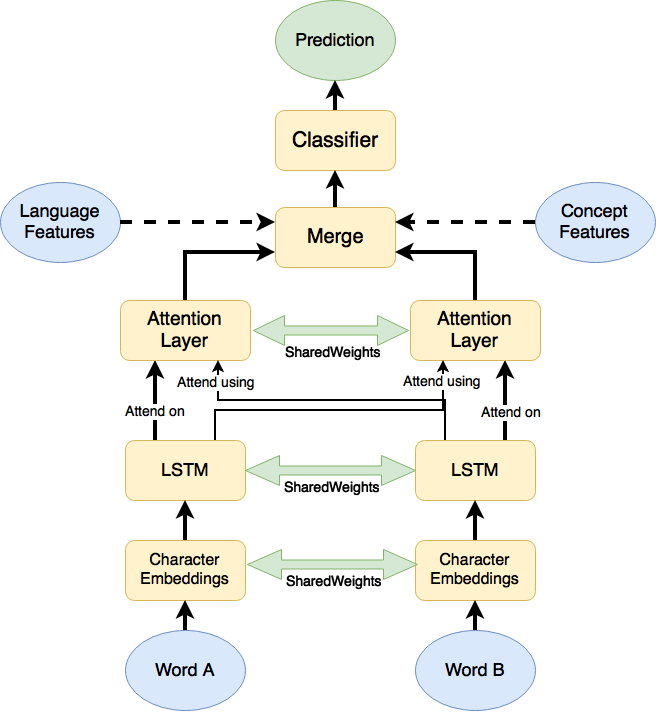
\includegraphics[width=0.45\textwidth]{CoAttNetwork}
    \caption{Recurrent Co-Attention Network for Cognate Discovery}
    \label{CoAttNet}
\end{figure}

The overall model used in our system is called the Recurrent Co-Attention Model (\textit{CoAtt}). It is adapted from the word-by-word attention model used by \cite{rocktaschel2016reasoning} for the task of recognising textual entailment (RTE) in natural language sentences. Just as the RTE task involves understanding the semantics of a sentence which is hidden behind sequence of words, the cognate identification task also requires information beyond surface character similarity, which was the motivation to adapt this particular model for our task. The network is illustrated in Figure~\ref{CoAttNet}. We have converted the RTE model into a siamese-style network that encodes a word pair in parallel and then makes a discriminative judgement in the final layer. 

The input words are first encoded into character level embeddings followed by a bidirectional LSTM network and finally a character by character attention layer as described the subsections that follow. The encodings of both the words are merged and passed through a 2-layer neural network with \textit{tanh} and \textit{sigmoid} activations to make a final binary prediction. Additionally we also add a \textit{Language features} vector or a \textit{Concept features} vector to the model by concatenating it with the merged attention vector before passing it to the 2-layer neural network.

%%%%%%%%%%%%%%%%%%%%%%
\subsection{Character Embeddings}

The input words are first encoded into character level embeddings. Character embeddings are a form of distributional representation, where every character of the vocabulary is expressed as a vector in a vector space. This is done using a character level embedding matrix $E \in \mathbb{R}^{n_e \times |C|}$. Here $n_e$ is the dimensionality of the embeddings and $C$ is the vocabulary of all characters. Thus for an input word $x$ which can be represented as sequence of characters $x = \{c_{i_1}, c_{i_2}, ..., c_{i_n}\}$, is transformed into a sequence of vectors $y = \{e_{i_1}, e_{i_2}, ..., e_{i_n}\}$ where $e_j$ is the $j^{th}$ column of the $E$ matrix. This embedding matrix is learnt during training and each column in the matrix represents the embedding vector of the respective token in the vocabulary. 

\cite{rama2016siamese} manually defined the character embeddings using various properties of the respective phoneme and fixed these embeddings during training. However, we observe that such a method restricts the power of the distributional representation to world knowledge known to us and letting the embeddings be learnt themselves should help learn a representation that is tuned for the task in hand. Thus, we use Rama's manually defined embeddings as an initialisation for the character embeddings and let these weights be trained during learning. It is found that such a method of embedding initialisation results in a better traning of the model as compared to a random initialisation.

%%%%%%%%%%%%%%%%%%%%%%
\subsection{LSTM network}

Recurrent Neural networks (RNN) with Long Short-Term Memory (LSTM) have been extensively been used in several NLP tasks. After the input words to the network are encoded using the character embedding matrix, we transform them use LSTM cells. Given the input words $y = \{e_1, e_2, ..., e_n\}$, at every time step $t$ the LSTM of hidden unit size $n_h$ uses the next input $e_t$, the previous output $h_{t-1}$ and the previous cell state $c_{t-1}$ to compute the next output $h_t$ and the next cell state $c_t$ as follows,

\begin{align}
H &= [e_t h_{t-1}] \\
i_t &= \sigma (W^iH + b^i) \\
o_t &= \sigma (W^oH + b^o) \\
f_t &= \sigma (W^fH + b^f) \\
c_t &= i_t * tanh(W^cH + b^c) + f_t * c_{t-1} \\
h_t &= o_t * tanh(c_t)
\end{align}

Here $W^i$, $W^o$, $W^f$, $W^c \in  \mathbb{R}^{n_e+n_h \times n_h}$ and $b_i$, $b_o$, $b_f$, $b_c \in \mathbb{R}^{n_h}$ are trained weights of the LSTM. The final output of the LSTM gives us a sequence $\{h_1, h_2, ..., h_n\}$ for every word, where $h_j \in \mathbb{R}^{n_h}$.

%%%%%%%%%%%%%%%%%%%%%%
\subsection{Attention}

Attention neural networks have been used extensively in tasks like machine translation \texttt{mtattention}, image captioning \texttt{cpattention} and visual question answering \texttt{stackedattention}. The attention mechanism helps to enhance the representation obtained from the LSTM cell state by giving it context that is used for attending. More precisely, we attend over the LSTM encoding of a given word, using a single characted encoding of the second word, which helps to generate a weighted representation of the first word that includes its important segments with respect to its similarity with the second word's character. 

Given a character vector $h \in  \mathbb{R}^{n_h}$ using which we would like to attend on a sequence of character vectors $Y = \{c_1, c_2, ..., c_L\} \in \mathbb{R}^{n_h \times L}$, we generate a set of attention weights $\alpha$ and a attention-weight representation $r \in  \mathbb{R}^{n_h}$ of $Y$ as,

\begin{align}
M &= tanh(W^yY + W^hh*e_L) \\
\alpha &= softmax(w^TM) \\
r &= Y\alpha_t^T
\end{align}

Using the mechanism followed by \cite{rocktaschel2016reasoning} for word-by-word attention, we employ a character-by-character attention model, wherein we find an attention weighted representation of the first word $Y = \{c_1, c_2, ..., c_L\} \in \mathbb{R}^{n_h \times L}$ at every character of the second word $H = \{h_1, h_2, ..., h_N\} \in \mathbb{R}^{n_h \times N}$.

\begin{align}
M_t &= tanh(W^yY + (W^hh_t + W^rr_{t-1})*e_L) \\
\alpha_t &= softmax(w^TM_t) \\
r_t &= Y\alpha_t^T + tanh(W^tr_{t-1})
\end{align}

Here $W^y$, $W^h$, $W^r$, $W^t \in  \mathbb{R}^{n_h \times n_h}$ and $w \in \mathbb{R}^{n_h}$ are trained weights of the Attention layer. The final output gives us $r_N = r_{YH}$ which can considered as attention weighted representation of $Y$ with respect to $H$. Similarly, we also obtain $r_{HY}$. The final feature vector $r^*$ that is passed to the multi-layer perceptron for classification is the concatenation of these 2 vectors.

\begin{align}
r^* &= [r_{HY} r_{YH}]
\end{align}

 This method of making both the sequences attend over each is called the \textit{Co-Attention} model.
 
%%%%%%%%%%%%%%%%%%%%%%
\subsection{Language Features}

It is known that some languages are more closely related to each other as compared to other languages. Thus, these languages which are closer would naturally tend to share more cognate pairs than they do with other languages. \cite{rama2016siamese} tried to exploit this information about language \textit{relatedness} by providing the network with 2-hot encoding vector that represents the respective languages of the 2 input words being tested. The network would then use this information about the languages to learn which language pairs may be more related using the training data provided.

Since we would primarily work in a Cross Language mode of evaluation, where the training and testing languages come from exclusive sets, it is intuitive that such \textit{Language Features} will not help to improve of the model in such a setting. Since the languages of the training and testing set do not overlap, the relevant language feature weights for the test set are never learnt. Any information about the affinity or interaction between the languages in the training set is not useful for the languages in the testing set. 

The \textit{Language Features} are thus only used during the Cross Concept mode of evaluation, where there is an overlap in the training and testing languages. We follow the same approach used by \cite{rama2016siamese} and provide the model with these addition \textit{Language Features} before the final classification by the 2-layer MLP. The 2-hot input language pair vector $x_{lang}$ is concatenated with the attention weighted representation of the input words $h^{*}$, before being fed into the final multi-layer perceptron for classification.

%%%%%%%%%%%%%%%%%%%%%%
\subsection{Concept Features}

As the information about the language of the input words can be beneficial for the task of cognate discovery, we hypothesise that information regarding the semantics or the meaning of the input word pair should also be helpful. The word semantics can provide information like the POS category of the word, which can be an useful if some POS classes show higher degree of variation in cognates while others show less.

We implement this by using GloVe word embeddings \cite{pennington2014glove}. Word embeddings are distributional representation of words in a low-dimensional space compared to the vocabulary size and they have been shown to capture semantic information about the words inherently. We use the GloVe embedding for the English concept of the word pair as obtained from the label in the dataset, and input this vector to the network before the final MLP for classification. The word embedding of the concept $x_{concept}$ is concatenated with the attention weighted representation of the input words $h^{*}$, before being fed into the final multi-layer perceptron for classification.

%%%%%%%%%%%%%%%%%%%%%%%%%%%%%%%%%%%%%%%%%%%%%%%%
\section{Experiments}

We primarily follow a Cross Language evaluation procedure, where the training and testing sample pairs are created using exclusive sets of languages. A random set of 70\% of the languages is set as the training set of languages and the rest as testing set. Both words in a sample pair belongs to the same concept or meaning. A word pair is assigned a positive cognate label if their cognate class ids match. The number of sample pairs obtained for training and testing from the different datasets formed using cross language evaluation test can be found in Table~\ref{CL_count}. 

We conducted ablation tests to study the contribution of different features and conducted tests on how the different levels of transcription affects the performance of the models. In the subsections below we describe the results from these different tests.

%%%%%%%%%%%%%%%%%%%%%%%%
\subsection{Evaluation Metric}

We report the \textit{F-score} and the area under the PR curve (\textit{AUC}) as a measure of performance for all the models. \textit{F-score} is computed as the harmonic mean of the \textit{precision} and \textit{recall}\footnote{Precision and Recall is computed on positive labels at 0.5 threshold. Precision = TP/(TP+FP), Recall = TP/(TP+FN), TP: True Positives, FP: False Positives, FN: False Negatives}. Since the dataset is heavily biased and contains a majority of negative cognate sample pairs, we do not use \textit{accuracy} as a measure of performance.

%%%%%%%%%%%%%%%%%%%%%%%%
\begin{table*}[t]
\centering
\begin{tabular}{lcccccc}
\multicolumn{1}{c}{\textbf{}} & \multicolumn{2}{c}{\textbf{Indo-European}} & \multicolumn{2}{c}{\textbf{Austronesian}} & \multicolumn{2}{c}{\textbf{Mayan}} \\
\multicolumn{1}{c}{}          & Total               & Positive             & Total               & Positive            & Total           & Positive         \\
Training Samples              & 218,429             & 56,678               & 333,626             & 96,356              & 25,473          & 9,614            \\
Testing Samples               & 9,894               & 2,188                & 20,799              & 5,296               & 1,458           & 441             
\end{tabular}
\caption{Data size for Cross Language Evaluation}
\label{CL_count}
\end{table*}

\begin{table*}[t]
\centering

\begin{tabular}{lcc}
\multicolumn{1}{c}{\multirow{2}{*}{\textbf{Model}}} & \multicolumn{2}{c}{\textbf{Indo-European}} \\ \cline{2-3} 
\multicolumn{1}{c}{}                                & \textit{F-Score}      & \textit{AUC}       \\ \hline
Gap-Weighted Subsequence                            & 59.0                  & 75.5               \\
PhoneticCNN                                         & 73.7                  & 86.1               \\
CharacterCNN                                        & 75.3                  & 85.3               \\
LSTM + No Attention                                 & 56.7                  & 59.0               \\
LSTM + Uniform Attention                            & 52.8                  & 59.4               \\ \hline
Co-Attention Model                                  & 83.8                  & 89.2               \\
\quad + IE                                          & 85.1                  & 92.4               \\
\quad + IE + CF                                     & \textbf{86.2}         & \textbf{93.0}     
\end{tabular}

\label{CL_res}
\caption{Cross Language Evaluation Results for Indo-European Dataset \newline [IE: \textit{Initialised Embeddings}, CF: \textit{Concept Features}]}
\end{table*}
%%%%%%%%%%%%%%%%%%%%%%%%
%%%%%%%%%%%%%%%%%%%%%%%%
\subsection{Baseline Models}

We compare our model against the following baseline models. 

\textbf{Gap-weighted Subsequences} : This model refers to the common subsequence model \cite{rama2015automatic} mentioned earlier. The author uses a string kernel based approach wherein he defines a vector for a word pair using all common subsequences between them and weighting the subsequence by their gaps in the strings.

\textbf{Phonetic CNN \& Character CNN} : These models are variations of the siamese-style CNN-based models \cite{rama2016siamese}. The models are inspired from CNN networks used for image-similarity tasks. The \textit{Phonetic CNN} model uses the manually defined (fixed) character embeddings in the network, whereas the \textit{Character CNN} model uses a 1-hot encoding to represent the different characters. The results reported for these models were found by rerunning the original code from the  author on the prepared datasets\footnote{It can be noted that there is a difference in the reported f-score of the CNN models as compared to the original paper. This is because we report the f-score with respect to the positive labels only, whereas the original paper reported the average f-scores of positive and negative labels (Observed from the implementation in author's code)}.

\textbf{LSTM + No Attention \& LSTM + Uniform Attention} : We also introduced two sanity-check baseline models to test the attention layer of the \textit{CoAtt} model. The \textit{LSTM + No Attention} model removes the Co-Attention layer from the \textit{CoAtt} model, while the \textit{LSTM + Uniform Attention} model does a simple average rather than a weighted average in the attention layer.

%%%%%%%%%%%%%%%%%%%%%%%%
\begin{table*}[t]
\centering
\begin{tabular}{lcccc}
\multicolumn{1}{c}{\multirow{2}{*}{\textbf{Model}}} & \multicolumn{2}{c}{\textbf{Austronesian}} & \multicolumn{2}{c}{\textbf{Mayan}} \\ \cline{2-5} 
\multicolumn{1}{c}{}                                & \textit{F-Score}      & \textit{AUC}      & \textit{F-Score}  & \textit{AUC}   \\ \hline
Gap-Weighted Subsequence                            & 58.8                  & 68.9              & 71.8              & 81.8           \\
PhoneticCNN                                         & 54.6                  & 68.0              & 72.8              & 85.0           \\
CharacterCNN                                        & 62.2                  & 71.6              & 75.9              & 85.7           \\ \hline
Co-Attention Model                                  & 69.0                  & 77.5              & 67.1              & 67.7           \\
\quad + IE                                          & 70.2                  & 79.3              & 63.6              & 71.3           \\
\quad + IE + CF                                     & \textbf{70.5}         & \textbf{79.7}     & 81.5              & 89.0           \\
\quad + IE + PreT (Indo-European)                   & -                     & -                 & 82.5              & 90.6           \\
\quad + IE + PreT (Austronesian)                    & -                     & -                 & \textbf{83.5}     & \textbf{91.2} 
\end{tabular}
\caption{Cross Language Evaluation Results for Austronesian and Mayan Datasets \newline [IE: \textit{Initialised Embeddings}, CF: \textit{Concept Features}, PreT: \textit{Pre-Training on another dataset}]}
\label{CL_res_2}
\end{table*}
%%%%%%%%%%%%%%%%%%%%%%%%
%%%%%%%%%%%%%%%%%%%%%%%%
\subsection{Experiments with Indo-European}

As can be observed in Table~\ref{CL_res}, the \textit{CoAtt} model performs significantly better than the CNN and the subsequence based models. The \textit{LSTM + No Attention} and \textit{LSTM + Uniform Attention} models reflect the importance of the attention layer adapted from the RTE model in the network, as without it the model does not perform very good. 

A few additional features added to the \textit{CoAtt} model helps to improve it even further. Initialising the character embeddings with the manually defined vectors (\textit{+ IE} models) increases the \textit{AUC} by around 3\%. Further, addition of the \textit{Concept features} discussed earlier, is also found to be useful (\textit{+ CF} model).

%%%%%%%%%%%%%%%%%%%%%%%%
\subsection{Experiments with Multiple Datasets}

Table~\ref{CL_res_2} lists the results of the models on these datasets. We observe a similar trend for the models on the Austronesian and Mayan datasets as well. However, the \textit{CoAtt} model does not train well on the Mayan dataset directly. This poor performance on the Mayan dataset is associated with its small size. The Mayan dataset being significantly smaller than the other datasets, does not prove sufficient for training the \textit{CoAtt} network. We justify this hypothesis subsequently with the \textit{Cross-Family Pretraining} experiment. The \textit{Concept features} are again found useful to improve the \textit{CoAtt} model, especially on the Mayan dataset, where the extra information about the meaning of input word pair helps the model to cross the baseline results. 

%%%%%%%%%%%%%%%%%%%%%%%%
\begin{table*}[t]
\centering
\begin{tabular}{lcccccc}
\multicolumn{1}{c}{\textbf{}} & \multicolumn{2}{c}{\textbf{Indo-European}} & \multicolumn{2}{c}{\textbf{Austronesian}} & \multicolumn{2}{c}{\textbf{Mayan}} \\
\multicolumn{1}{c}{}          & Total               & Positive             & Total               & Positive            & Total           & Positive         \\
Training Samples              & 223,666             & 61,856               & 375,693             & 126,081             & 28,222          & 10.482           \\
Testing Samples               & 103,092             & 21,547               & 150,248             & 41,595              & 12,344          & 4,297           
\end{tabular}
\caption{Data size for Cross Concept Evaluation}
\label{CC_count}
\end{table*}

\begin{table*}[t]
\centering
\begin{tabular}{lcccccc}
\multicolumn{1}{c}{\multirow{2}{*}{\textbf{Model}}} & \multicolumn{2}{c}{\textbf{Indo-European}} \\ \cline{2-3} 
\multicolumn{1}{c}{}                                & \textit{F-Score}      & \textit{AUC}    \\ \hline
Gap-weighted Subsequence                            & 51.6                  & 62.0            \\ \hline
PhoneticCNN + Language Features                     & \textbf{66.4}         & \textbf{73.2}   \\
CharacterCNN + Language Features                    & 63.5                  & 70.5            \\ \hline
CoAtt                                               & 64.8                  & 69.8            \\
CoAtt + Language Features                           & 65.6                  & 70.8            \\
CoAtt+ Concept Features                             & 64.1                  & 70.6            \\
CoAtt + Pre-training (Austro)                       & 65.8                  & 71.0 
\end{tabular}
\label{CC_res}
\caption{Cross Concept Evaluation Results for Indo-European}
\end{table*}
%%%%%%%%%%%%%%%%%%%%%%%%

%%%%%%%%%%%%%%%%%%%%%%
\subsubsection*{Cross Family Pre-training Experiments}

The three different language families with which we work have completely different origins and are placed across different regions geographically. We test if any notion of language evolution is still shared amongst these independently evolved families. This is done through the joint learning of models. The network is instantiated with the combined character vocabulary of two datasets. Then the model is trained on one dataset till the loss saturated. This is followed by the training on a second dataset, starting from the weights learned from the pre-training. 

It is found that such a joint-training procedure helps the \textit{CoAtt} model on the Mayan dataset significantly. The pretraining procedure is able to provide a good initialisation point to start training on the Mayan dataset. The pretrained models perform significantly better than the baseline models (\textit{PreT} models in Table~\ref{CL_res_2}). This also provides evidence to support our hypothesis that the \textit{CoAtt} was not able to learn on the Mayan dataset because of lack of enough data to train the network, but pre-training the model on other language families helped to show the true potential of the model on the dataset.

%%%%%%%%%%%%%%%%%%%%%%%%
\subsection{Cross Concept Evaluation}

We also conducted cross-concept evaluation experiments, where the training and testing datapoints were formed using exclusive sets of \textit{concepts} or \textit{meanings}. For this, we followed the same scheme as done by \cite{rama2016siamese}, wherein we took the first 70\% of the concepts as training concepts and the remaining concepts as testing concepts. The training and testing set size details formed using cross concept evaluation test can be found in Table~\ref{CC_res}. The results for the cross concept evaluation tests are listed in Table~\ref{CC_res}.

It is observed that the \textit{CoAtt} model is able to reach close to, but not improve on, the performance of the \textit{PhoneticCNN + Language Features} model for the Indo-European dataset. In fact, the \textit{CoAtt} model with pre-training and extra features reaches the performance of the \textit{CharCNN + Lang} model, but the \textit{PhoneticCNN + Lang} still leads by 3 points.

The cross-concept evaluation test can be thought of as a more rigorous test for cognate detection as the models have not seen any of the similar word structures during training. Words coming from different concepts would have different sequence structures altogether and for a model to predict cognate similarity in such a case would definitely have to exploit phoneme similarity information in the context of cognates.

%%%%%%%%%%%%%%%%%%%%%%%%%%%%%%%%%%%%%%%%%%%%%%%%
\section{Analysis}

\subsection{Concept Wise Performance}

In this analysis of the models, we looked at the performance of various models over the individual concepts in the test set samples. It is observed that the performance of \textit{CoAtt} is more uniform throughout the concepts as compared to more varied distribution of the subsequence model. For concepts like WHAT, WHO, WHERE, HOW, THERE where the subsequence model performed poorly, the \textit{CoAtt} model is able to acheive high scores. The \textit{CoAtt} model performs poorly on a few selected concepts like AT, IF, IN, BECAUSE, GIVE. By looking at the samples, it is found that these concepts are heavily biased by negative samples and contain only a handful of positive cognate pair examples. In fact the subsequence model could not perform at all on these concepts as the highly biased data is coupled with almost no overlap of subsequences.

\begin{table}[h]
\centering
\begin{tabular}{ccc}
\textbf{Concept} & \textbf{CoAtt} & \textbf{Subseq} \\ \hline
WHAT             & \textit{0.91}  & \textit{0.04}   \\
WHO              & \textit{0.85}  & \textit{0.05}   \\
WHERE            & \textit{0.90}  & \textit{0.16}   \\
HOW              & \textit{0.90}  & \textit{0.17}   \\
THERE            & \textit{0.95}  & \textit{0.19}  \\
GIVE             & \textit{0.45}  & \textit{0.35}  \\
BECAUSE          & \textit{0.28}  & \textit{0}      \\
IN               & \textit{0.35}  & \textit{0}      \\
IF               & \textit{0.31}  & \textit{0}      \\
AT               & \textit{0.25}  & \textit{0}      
\end{tabular}
\caption{\textit{CoAtt} vs \textit{Subseq} model on various concepts (F-Score)}
\end{table}

\subsection{Transcription Tests}

As mentioned in an earlier section, the Indo-European dataset is available to us different transcriptions. The dataset is trascribed in ASJP like the other datasets and is also transcribed in IPA, which is a much finer representation as compared to ASJP. On comparing the models trained on these different transcriptions of the same data, it is found that the IPA model performs poorly on some concepts like GUTS, SWIM, WIPE, WHITE, SING where the ASJP model gives good results. On the other hand, the IPA model performs relatively better on concepts like FIRE, SLEEP, PULL, SAY and SMOOTH. By looking at specific examples, we find that for concepts like FIRE and PULL, the ASJP model gives many false positives which can be a fault due to the coarser representation of the ASJP character.

\begin{table}[h]
\centering
\begin{tabular}{ccc}
\textbf{Concept} & \textbf{IPA}  & \textbf{ASJP} \\ \hline
GUTS             & \textit{0.28} & \textit{0.58} \\
SWIM             & \textit{0.47} & 0.93          \\
WHITE            & \textit{0.54} & \textit{0.75} \\
WIPE             & \textit{0.55} & \textit{0.72} \\
SING             & \textit{0.56} & \textit{0.88} \\ \hline
FIRE             & \textit{0.62} & \textit{0.33} \\
SLEEP            & \textit{0.73} & 0.39          \\
PULL             & \textit{0.83} & \textit{0.50} \\
SMOOTH           & \textit{0.83} & \textit{0.50} \\
SAY              & \textit{0.90} & \textit{0.51}
\end{tabular}
\caption{\textit{CoAtt} model using IPA vs ASJP transcription on various concepts (F-Score)}
\end{table}

\begin{figure}[t]
\centering
  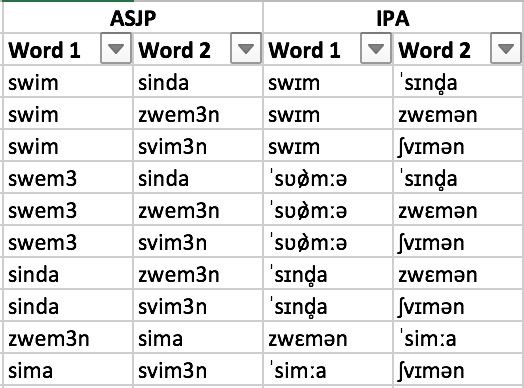
\includegraphics[width=.9\linewidth]{swim}
  \caption{Sample test word pairs from the concept SWIM}
  \label{disssim}
\end{figure}

Figure 2 shows few test sample pairs from the concept SWIM. It is observed that for all of these samples, the IPA model falsely predicts negatives whereas the ASJP model is correctly able to predict them all as cognates. Here perhaps the very find representation in IPA throws the model's judgment off and its not able to pick up the correspondence correctly. It is also interesting to note that for all of these samples, adding the \textit{concept feature} of SWIM to the \textit{CoAtt + Concept Features} model makes it predict all of them as cognates. Thus, perhaps adding the concept features signals the model to relax the degree of overlapping of phonemes and become less strict in predicting cognates.

\subsection{Hindi-Marathi Domain Adaptation}

Finally we applied the \textit{CoAtt} model to the domain of Hindi-Marathi. The model was trained on the IELex dataset with IPA transcription with a character vocabulary of around 150 phonetic characters. The model was trained in a cross-language evaluation style. It should be noted that the IELex database contains instances from Marathi, but it does not directly contain instances from Hindi. However, it does contain words from Urdu and Bhojpuri (Bihari) which are also languages closely related to Hindi and share many words of the vocabulary with Hindi.

We used the TDIL sentence-aligned corpus. The corpus contains sentences from Hindi-Marathi that are POS tagged and transcribed in Devanagari. We specifically extracted word pairs from each sentence with the NOUN and VERB tags. Since the sentences are not word aligned, we extracted candidate word pairs for testing by choosing the first word with the same tag in either sentence as the candidate pair. The words were converted from Devanagari to IPA using a rule-based system and finally fed into the model. We extracted 16K pairs from Nouns and 9K pairs from Verbs.

On first observation it seems that the model is doing a fair job of aligning similar word pairs that are possibly cognates. We tested the performance of the model by randomly sampling 50 word pairs each from NOUNs and VERBs and manually annotating them. We found that our model gives an 80\% accuracy on Verbs and 74\% accuracy on Nouns. The model is able to find word pairs with a common stem without the need of lemmetization. In the case of verbs, it can be observed that the model is able to see through the inflections on the verbs to predict the pairs with similar stems as cognates. 

%%%%%%%%%%%%%%%%%%%%%%%%%%%%%%%%%%%%%%%%%%%%%%%%
\section{Conclusion}

The task of cognate discovery dwells into domain of finding rich hidden representation for words. It is found that simple surface similarity measures like common subsequence based features fail to capture the essence of phonological evolution and sound correspondences. Where there is large drift in the word structures and the characters of the words, these methods fail to capture any similarity between the words. Deep learning models like LSTMs are able to exploit such features to make better judgments on the prediction task. 

Cognate formation results from the evolution of sound changes in the words over time. From our experiments we have seen that there is a link in this evolution of sound class with the semantics of the words. Because words with different meanings are used in different frequencies, some appear to go through rapid adaptation and while others do not change by a lot. The models generally perform better on Nouns and Adjective words and they also have more number of cognate classes. In particular, words like \textit{`WHAT'}, \textit{`WHEN'}, \textit{`HOW'} show a lot of variation even within a cognate class, so much that some cognate word pairs do not share any subsequence. Introducing concept features to the models in the form of word embeddings is seen to help in improving the results. It is also found that joint training of the models with data from different language families is also useful.

By using deep learning models, the performance boosts are enough to test the model in an open domain. We applied our model to the Hindi-Marathi domain and found that the model is able to segregate the word pairs efficiently. 

%%%%%%%%%%%%%%%%%%%%%%%%%%%%%%%%%%%%%%%%%%%%%%%%
\bibliography{tacl}
\bibliographystyle{acl2012}

\end{document}


